\documentclass[17pt,a0paper,landscape,
  margin=0mm,
  innermargin=10mm,
  blockverticalspace=6mm,
  colspace=8mm]{tikzposter}

\usepackage[utf8]{inputenc}
\usepackage[T1]{fontenc}
\usepackage{amsmath,amssymb,amsfonts,booktabs,graphicx}
\usepackage{tikz}
\usepackage{pgfplots}
\usepackage{xcolor}
\usepackage{enumitem}
\usepackage{qrcode}
\pgfplotsset{compat=1.18}
\usetikzlibrary{arrows.meta,positioning,calc,decorations.pathreplacing}

\usetheme{Default}
\useblockstyle{Default}
\usetitlestyle{Filled}

% ---------------- Colours (same palette as the figures) ----------------
\definecolor{posterNavy}{RGB}{18,45,85}
\definecolor{posterTeal}{RGB}{0,120,125}
\definecolor{posterOrange}{RGB}{218,115,45}
\definecolor{posterGold}{RGB}{200,160,40}
\definecolor{posterPurple}{RGB}{120,80,160}
\definecolor{posterGrey}{RGB}{244,247,250}
\definecolor{posterLightBlue}{RGB}{232,241,248}
\definecolor{posterText}{RGB}{25,25,25}

\definecolorpalette{CleanBlue}{
  \definecolor{colorOne}{named}{posterNavy}
  \definecolor{colorTwo}{named}{posterTeal}
  \definecolor{colorThree}{named}{posterGrey}
}
\usecolorpalette{CleanBlue}
\colorlet{backgroundcolor}{posterGrey}
\colorlet{framecolor}{posterNavy}
\colorlet{titlebgcolor}{posterNavy}
\colorlet{titlefgcolor}{white}
\colorlet{blocktitlebgcolor}{posterTeal}
\colorlet{blocktitlefgcolor}{white}
\colorlet{blockbodybgcolor}{white}
\colorlet{blockbodyfgcolor}{posterText}

% ---------------- Commands ----------------
\newcommand{\w}{\mathbf{w}}
\newcommand{\mub}{\boldsymbol{\mu}}
\newcommand{\Sig}{\boldsymbol{\Sigma}}
\newcommand{\E}{\mathbb{E}}
\newcommand{\R}{\mathbb{R}}
\newcommand{\model}[1]{\textbf{\color{posterNavy}#1}}
\newcommand{\statement}[1]{\par\vspace{0.25em}\noindent\textbf{\color{posterNavy}#1}\par\vspace{0.25em}}

\newcommand{\insightbox}[1]{%
\vspace{0.15cm}
\begin{center}
\setlength{\fboxsep}{6pt}
\fcolorbox{posterOrange}{posterLightBlue}{
\begin{minipage}{0.93\linewidth}
\centering #1
\end{minipage}}
\end{center}
\vspace{-0.1cm}
}

\setlist[itemize]{leftmargin=1.1em,itemsep=0.1em,topsep=0.1em}
\setlist[enumerate]{leftmargin=1.4em,itemsep=0.1em,topsep=0.1em}

% ---------------- Title ----------------
\title{
\parbox{\linewidth}{
\centering
\Huge\textbf{Does the Risk Model Still Matter Once the Investor's Rules Are In?}
}}
\author{Yeshwanth Patil, Liu Bowen, Kenta Ueda, Jia Qi Choy, Mana Okujo}
\institute{Blend-Ed}

\begin{document}

\maketitle[
width=\paperwidth,
titletotopverticalspace=0mm,
titletoblockverticalspace=4mm
]

\begin{columns}

% ============================================================
% COLUMN 1
% ============================================================
\column{0.333}

\block{Background}{
Anyone investing money faces one decision: how much to put in each asset. Portfolio optimisation answers it by estimating each asset's expected return and risk from past prices and solving for the best mix. Two things go wrong in practice. The estimates come from a few years of noisy history, so the ``best'' mix is only as good as its inputs. And real investors add rules the textbook ignores: hold no more than a dozen names, keep some cash, cap any one sector, pay for every trade.

\statement{Real-world investing imposes constraints on portfolio optimisation. We ask how the choice of risk model changes the outcome once those constraints are fixed, and whether any model earns its complexity over the simplest alternative, equal weight.}

\textbf{What we ran.} Five investor rule-sets $\times$ five risk models (Markowitz, Markowitz with Ledoit--Wolf shrinkage, robust, CVaR, equal weight), each managed through the same walk-forward backtest over 2016--2025 with trading costs. Every tuning decision used 2011--2015 data only.

\textbf{Up front.} One decade, one market (US large caps), no short selling or leverage. The universe is chosen with hindsight: all 40 names still trade today, which flatters every strategy equally but not the comparison between them.
}

\block{1. Data and Investor Rule-Sets}{
\begin{itemize}
\item \textbf{Universe:} 40 US large caps (four largest per GICS sector at end-2015), a bond ETF (AGG), gold (GLD), cash (3-month T-bill).
\item \textbf{Prices:} daily, 2008--2025. Tuning period 2011--2015, test period 2016--2025.
\item \textbf{Rule-sets:} five investor archetypes; each is one row below. Values derived from Vanguard LifeStrategy and target-date allocations and the 2022 Survey of Consumer Finances.
\end{itemize}
\begin{center}
\begin{tabular}{lccccc}
\toprule
Archetype & CVaR limit & max & $w_{\max}$ & cash & sector \\
          & start$\to$end & holdings & & floor & caps \\
\midrule
Preserver   & 1.0$\to$0.5\% & 20 & 8\%  & 10\% & IT 20\%, Energy 10\% \\
Steady Hand & 1.5$\to$0.7\% & 15 & 10\% & 5\%  & -- \\
Builder     & 2.0$\to$1.0\% & 12 & 12\% & 2\%  & -- \\
Maverick    & 2.8$\to$1.4\% & 8  & 20\% & 0\%  & -- \\
Ethical     & 1.5$\to$0.7\% & 15 & 10\% & 5\%  & excl.\ tobacco, oil, defence \\
\bottomrule
\end{tabular}
\end{center}
}

\block{2. The Portfolio Problem}{
$n$ assets. The decision is $\w\in\R^{n}$, the fraction of the portfolio in each asset. $z_a\in\{0,1\}$ records whether asset $a$ is held; $b_a, s_a\ge 0$ are the amounts bought and sold relative to the current weights $\w^{\text{prev}}$. From the last $|S|$ trading days we estimate the expected daily return $\hat\mub$, the covariance $\hat\Sig$, and keep each day's return vector $r_s$.
{\large
\[
\max_{\w,\,z,\,b,\,s}\;\; h\,\hat\mub^{\top}\w \;-\; \tau\sum_a (b_a + s_a)
\qquad\text{subject to}\qquad \rho(\w)\;\le\;\rho_{\max}(t)
\]
\vspace{-0.4em}
\begin{align*}
\sum_a w_a = 1, \qquad w_a &= w^{\text{prev}}_a + b_a - s_a && \text{fully invested; trades add up} \\
w^{\min} z_a \;\le\; w_a &\le\; w^{\max}_a z_a, \qquad \sum_{a\,\notin\,\text{cash}} z_a \le K && \text{no tiny positions; at most $K$ names} \\
\sum_{a\in\text{sector }k} w_a &\le c_k, \qquad w_{\text{cash}} \ge c_{\min} && \text{sector caps; cash floor}
\end{align*}}
Return is scaled by the expected holding period $h$ (21 days) because the cost $\tau$ (10\,bp per unit traded) is paid once. The risk limit $\rho_{\max}(t)$ tightens linearly as the investor's horizon shrinks, like a target-date fund. The binaries $z_a$ make every model a mixed-integer programme. Only the risk term $\rho(\w)$ differs between models.
}

\block{3. Five Risk Models}{
\begin{itemize}
\item \model{Markowitz.} Variance. $\rho(\w) = \w^{\top}\hat\Sig\,\w$. The 1952 textbook. Quadratic; solved with Gurobi.
\item \model{Markowitz + Ledoit--Wolf.} Same $\rho$, but the covariance is shrunk toward a multiple of the identity,
{\large $\hat\Sig_{\text{LW}} = (1-\delta)\hat\Sig + \delta\bar\sigma^{2} I$}, with $\delta$ chosen to minimise expected estimation error. Fixes the covariance.
\item \model{Robust.} Treats $\hat\mub$ as uncertain: the true mean lies in an ellipsoid around it, and the objective becomes the worst case in that set,
{\large $\hat\mub^{\top}\w - \kappa\sqrt{\w^{\top}\Omega\,\w}$}, $\Omega = \hat\Sig/|S|$. Fixes the mean. Second-order cone; Gurobi.
\item \model{CVaR.} Replaces variance with the mean loss on the worst $(1-\alpha)$ share of days, $\alpha=0.95$. Rockafellar--Uryasev make this linear with a threshold $\zeta$ (the VaR) and one excess-loss variable $u_s$ per historical day:
{\large\[
\rho(\w) = \zeta + \frac{1}{(1-\alpha)|S|}\sum_{s\in S} u_s,\qquad u_s \;\ge\; -\,r_s^{\top}\w - \zeta,\quad u_s \ge 0 .
\]}
No covariance, no distribution assumed. Linear; solved with HiGHS.
\item \model{Equal weight ($1/N$).} $w_a = 1/N$ over the permitted assets. Ignores the data and every rule except exclusions. The benchmark that optimisers must beat.
\end{itemize}
}

% ============================================================
% COLUMN 2
% ============================================================
\column{0.333}

\block{4. Why the Estimates Matter}{
Every model in box 3 runs on $\hat\mub$, $\hat\Sig$ or the scenarios $r_s$, all estimated from three years of history. Correlations of the 40 stocks, ordered by sector: what the window ending 31 Dec 2019 told the optimiser, and what the next three months delivered.
\begin{center}
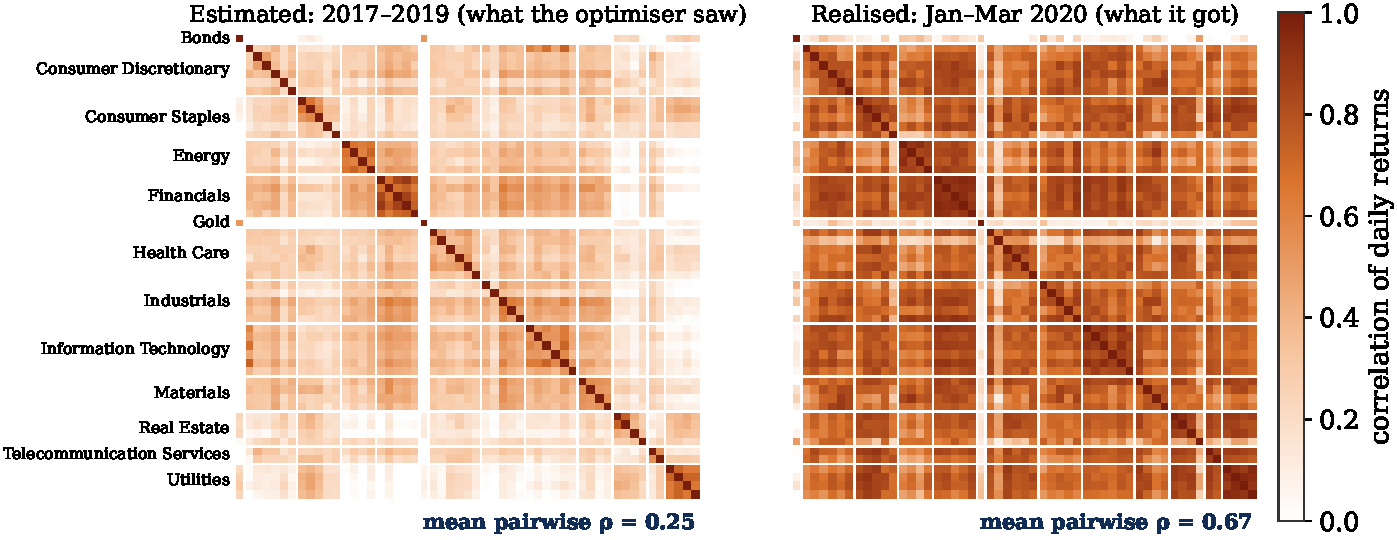
\includegraphics[width=0.88\linewidth]{figures/fig_corr.pdf}
\end{center}
\insightbox{One event turned every pairwise estimate wrong at once: mean correlation 0.25 $\to$ 0.67. Diversification is measured in calm markets and needed in crashes, when it is not there. Each risk model is a different hedge against this gap.}
}

\block{5. When the Portfolio Changes}{
The weights are re-solved (a new $\w$ from box 2, starting from the current $\w^{\text{prev}}$) when any of these holds, checked daily and at least 10 days apart:
{\large
\begin{align*}
&\text{calendar:} && \text{63 trading days since the last solve} \\
&\text{drift:} && \sum_a \bigl|w_a - w^{\text{target}}_a\bigr| \;\ge\; 0.10 \\
&\text{volatility regime:} && \sigma_{21}/\sigma_{252} \;\ge\; 2
\end{align*}}
$w^{\text{target}}$ is the last solved allocation, from which prices have since pulled the holdings; $\sigma_{21}, \sigma_{252}$ are the market's short- and long-run volatility. Each solve sees only the 756 trading days before it. The lookback, shrinkage and trigger levels were chosen on 2011--2015 by Sharpe ratio; 2016--2025 was never used for any design decision.

\textbf{Two implementation lessons.} (i) A trade costs 10\,bp once, but $\hat\mub$ is per day: without the factor $h$ in the objective no trade is ever worth it and the model sits in cash. (ii) Shrinking expected returns toward the average must skip cash, or cash looks like a stock.
}

\block{7. Conclusions and Limitations}{
\begin{itemize}
\item \textbf{The rules matter more than the model.} With holdings, position, sector and cash limits in place, four risk models land within 0.1 Sharpe of each other, well inside bootstrap noise. The rule-set, not the optimiser, sets the risk level.
\item \textbf{CVaR is the best optimiser and the cheapest} (a MILP, no covariance), but it does not beat $1/N$ on this decade.
\item \textbf{Robust optimisation is consistently worst}: guarding against the worst-case mean doubles up on rules that already limit concentration; tuning showed Sharpe falling monotonically in $\kappa$.
\item \textbf{Nothing beats the S\&P 500}: 2016--25 was a mega-cap tech decade and every rule-set caps exactly those names. What the optimisers bought was drawdown, not return.
\end{itemize}
\textbf{Limitations.} One decade, one market; survivorship bias; the CVaR$\to$variance translation assumes normality; $1/N$ inherits the exclusions but no other rule; no shorting or leverage.
\insightbox{Interactive version: pick an investor, travel back to 2016 and watch each model trade.\quad \qrcode[height=2.2cm]{https://example.org/}}
}

\block{References}{
\footnotesize
\setlist[itemize]{itemsep=0em}
\begin{itemize}
\item H. Markowitz. Portfolio selection. \emph{J. Finance}, 1952.
\item R. T. Rockafellar and S. Uryasev. Optimization of conditional value-at-risk. \emph{J. Risk}, 2000.
\item O. Ledoit and M. Wolf. A well-conditioned estimator for large-dimensional covariance matrices. \emph{J. Multivariate Analysis}, 2004.
\item V. DeMiguel, L. Garlappi and R. Uppal. Optimal versus naive diversification: how inefficient is the 1/N portfolio strategy? \emph{Rev. Financial Studies}, 2009.
\item D. Goldfarb and G. Iyengar. Robust portfolio selection problems. \emph{Math. Operations Research}, 2003.
\item D. N. Politis and J. P. Romano. The stationary bootstrap. \emph{J. Amer. Statist. Assoc.}, 1994.
\end{itemize}
}

% ============================================================
% COLUMN 3
% ============================================================
\column{0.334}

\block{6. Results: 25 Portfolios, One Decade}{
\begin{center}
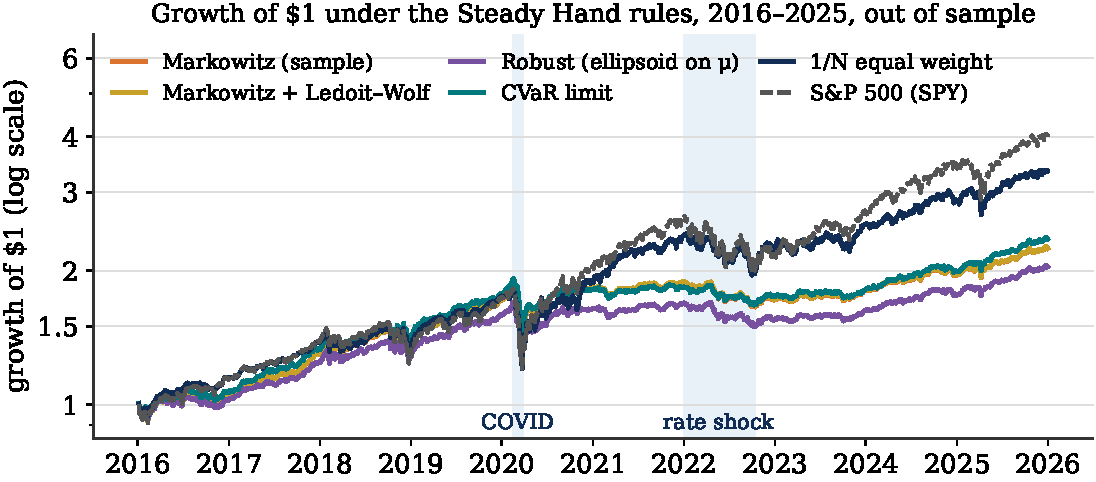
\includegraphics[width=0.99\linewidth]{figures/fig_growth.pdf}
\end{center}
\vspace{-0.25cm}
\begin{center}
\begin{minipage}[t]{0.495\linewidth}
\centering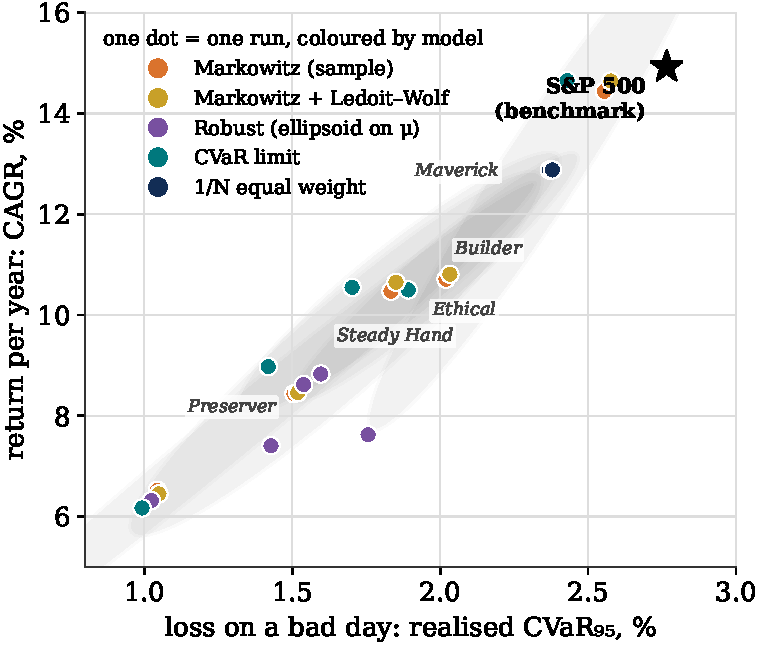
\includegraphics[width=\linewidth]{figures/fig_scatter.pdf}
\end{minipage}\hfill
\begin{minipage}[t]{0.495\linewidth}
\centering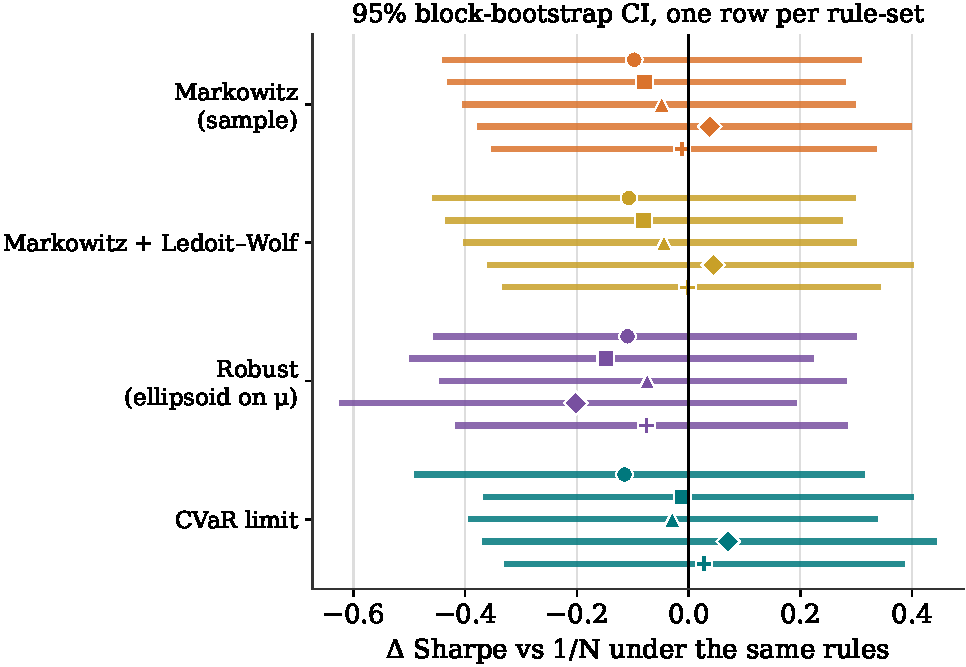
\includegraphics[width=\linewidth]{figures/fig_bootstrap_sharpe.pdf}
\end{minipage}
\end{center}
\textbf{Left:} runs cluster by \emph{rules} (marker), not by model (colour): the constraint set decides where a portfolio sits on the risk axis. \textbf{Right:} paired Sharpe difference against $1/N$ under the same rules; stationary block bootstrap, 5\,000 resamples, mean block 21 days. No interval clears zero.
\begin{center}
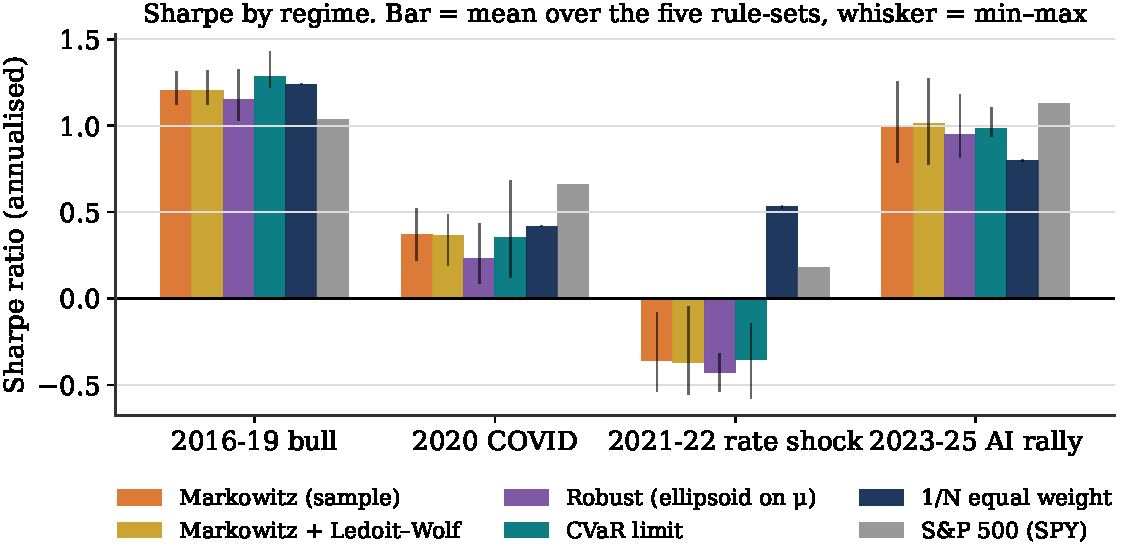
\includegraphics[width=0.99\linewidth]{figures/fig_subperiods.pdf}
\end{center}
\vspace{-0.15cm}
The models separate in one regime, \textbf{2021--22}: every optimiser is negative and $1/N$ is positive. With a 3-year lookback the optimisers had loaded up on the 2019--21 winners just before rates rose. Estimation error is momentum in disguise.
\begin{center}\small
\begin{tabular}{lcccc}
\toprule
Model & CAGR \% & Sharpe [95\% CI] & Max DD \% & CVaR$_{95}$ \% \\
\midrule
Markowitz (sample) & 10.1 & 0.67 [0.14, 1.35] & -25 & 1.79 \\
Markowitz + Ledoit--Wolf & 10.2 & 0.67 [0.14, 1.35] & -25 & 1.81 \\
Robust (ellipsoid on $\mu$) & 7.8 & 0.59 [0.03, 1.29] & -22 & 1.47 \\
CVaR limit & 10.2 & 0.70 [0.17, 1.40] & -25 & 1.69 \\
$1/N$ equal weight & 12.9 & 0.71 [0.19, 1.36] & -33 & 2.37 \\
S\&P 500 (SPY) & 14.9 & 0.74 [0.20, 1.38] & -34 & 2.77 \\
\bottomrule
\end{tabular}

\end{center}
\vspace{-0.15cm}
{\small Means over the five rule-sets. The optimisers trade 3--5 points of CAGR for $\approx$8 points less drawdown than $1/N$ at the same Sharpe: they delivered the risk target they were given.}
}

% ============================================================
% COLUMN 3
% ============================================================
\column{0.334}

\end{columns}
\end{document}
